\section{Project plan, methodology and management}
\label{sec:results}

As the project progresses, the focus will be on improving and optimising the algorithm for increased accuracy in tool wear detection. The design iteration will incorporate deep learning techniques, tailored through simulation models in the Python programming environment. Special attention will be given to the selection of features that correlate with wear patterns, utilizing a dataset comprised of high-resolution images and sensor data.

Simulations will be conducted to validate the model against established benchmarks of wear prediction, using libraries such as TensorFlow and PyTorch to ensure computational efficiency and scalability. Once the model demonstrates robust performance, a prototype algorithm will be deployed in a test environment to assess its real-world applicability.

In the initial data collection phase, our primary collaboration will be with Dr. Changhong and Dr. Xinyue. Our discussions will center around the accuracy and usability of the collected data, ensuring the foundations of our dataset are robust and reliable for subsequent analysis. This stage is critical for setting the precedent for the quality of our deep learning model.

As we progress into the intermediate and later stages of the project, we will engage in thorough discussions with Dr. Dongwang to refine our model. These discussions will aim to enhance the accuracy and reliability of the model while also considering computational efficiency. Dr. Dongwang’s expertise in algorithm optimization will be invaluable in achieving a balance between performance and speed, which is essential for real-time applications.

Throughout these phases, we will maintain a consistent and transparent communication channel with our collaborators to ensure that the project aligns with the overarching goals of precision and reliability.

The Gantt chart is shown below in Figure \ref{fig:gantt}.

\begin{figure}[htbp]
    \centering
    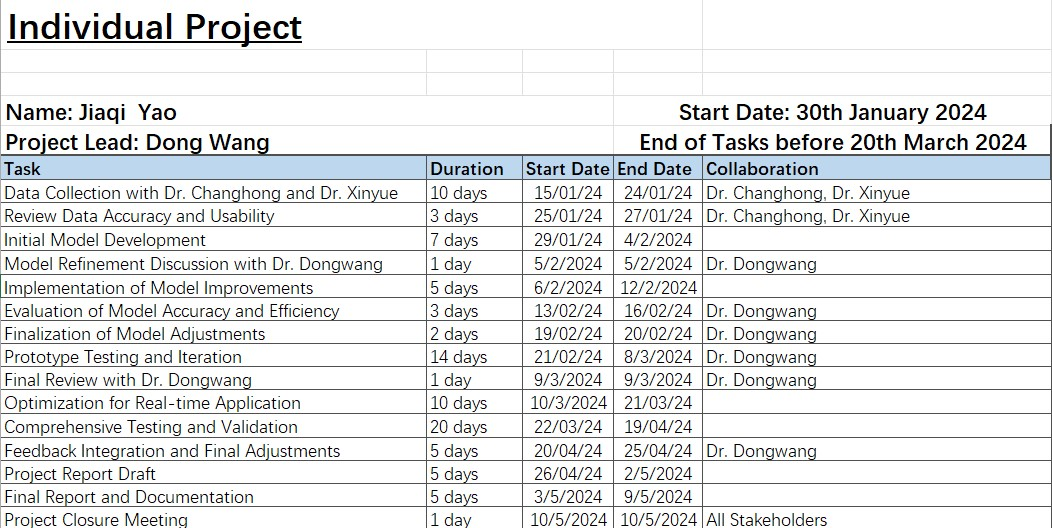
\includegraphics[width=\textwidth]{gantt.jpg}
    \caption{Gantt chart}
    \label{fig:gantt}
\end{figure}
\FloatBarrier % Now the table doesn't flow over to any other sections